% Primo periodo
\subsubsection{Primo periodo (8/11/2023 - 26/11/2023)}

\subsubsubsection{Planning}
\subsubsubsubsection*{Attività pianificate}
All'inizio del periodo ad ogni membro del gruppo sono stati assegnati ruoli specifici, di seguito riportati:
\begin{table}[H]
\centering
\begin{tabular}{|c|c|c|}
\hline
\textbf{Membro} & \textbf{Ruolo} \\
\hline
Samuele V. & Analista \\
\hline
Michele Z. & Verificatore \\
\hline
Leonardo B. & Amministratore \\
\hline
Riccardo Z. & Analista \\
\hline
Filippo T. & Responsabile \\
\hline
Davide B. & Progettista \\
\hline
\end{tabular}
\caption{Ruoli assunti per ciascun membro del team all'inizio del periodo}
\end{table}
\\
Gli obiettivi posti per lo sprint sono stati i seguenti:
\begin{itemize}
    \item Approfondire in collaborazione con il proponente le tecnologie da utilizzare e i requisiti del progetto;
    \item Iniziare il documento di \emph{Analisi dei Requisiti};
    \item Ideare un sistema di versionamento regolamentato per i documenti;
    \item Continuare \emph{Norme di Progetto}.
\end{itemize}

\subsubsubsubsection*{Preventivo}
\begin{table}[H]
    \centering
\begin{spreadtab}{{tabular}{|c|c|c|c|c|c|c|c|}}
    \hline
    @\textbf{Membro} & @\textbf{Re} & @\textbf{Amm} & @\textbf{An} & @\textbf{Progr} & @\textbf{Proge} & @\textbf{Ve} & @\textbf{Totale} \\
    \hline
    @ Samuele V.   & 0          & 0          & 3         & 0          & 0     & 0     & sum(b2:g2) \\
    @ Leonardo B.  & 0         & 1          & 0        & 0        & 0     & 0    & sum(b3:g3) \\
    @ Riccardo Z.  & 0          & 0          & 3          & 0          & 0     & 0   & sum(b4:g4) \\
    @ Davide B.    & 0          & 0          & 0       & 0       & 0     & 3     & sum(b5:g5) \\
    @ Michele Z.   & 0          & 0          & 0         & 0          & 0     & 4     & sum(b6:g6) \\
    @ Filippo T.   & 2          & 0          & 0         & 0          & 0     & 0     & sum(b7:g7) \\
    \hline
    @\textbf{Ore totali} & sum(b2:b7) & sum(c2:c7) & sum(d2:d7) & sum(e2:e7) & sum(f2:f7) & sum(g2:g7) &  sum(b8:g8)\\
    \hline
    @\textbf{Costo totale} & 30*b8 & 20*c8 & 25*d8 & 15*e8 & 25*f8 & 15*g8 & sum(b9:g9)\\
    \hline
\end{spreadtab}
    \caption{Preventivo orario ed economico parziale per il primo periodo, in base al ruolo}
    \label{tab:prev_rtb}
    \vspace{5mm}
    \textbf{Legenda:} \textit{Re} = Responsabile, \textit{Amm} = Amministratore, \textit{An} = Analista, \textit{Progr} = Programmatore, \textit{Proge} = Progettista, \textit{Ve} = Verificatore
\end{table}

\begin{figure}[H]
  \centering
  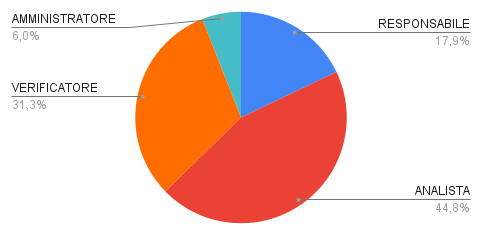
\includegraphics[width=0.6\linewidth]{grafici/1_periodo_torta.png}
  \caption{Ripartizione dei costi per ruolo nel $1^\circ$ periodo}
        \vspace{10mm}
  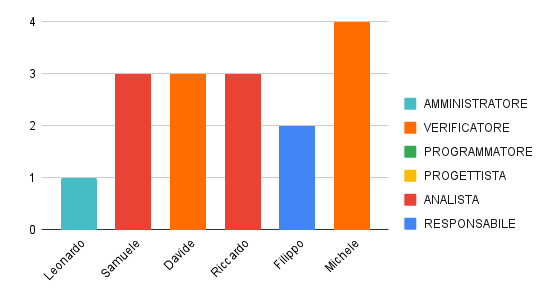
\includegraphics[width=0.7\linewidth]{grafici/1_periodo_istogramma.png}
  \caption{Ore preventivate per ciascuna persona nel $1^\circ$ periodo}
\end{figure}

\subsubsubsection{Review}
\subsubsubsubsection*{Attività svolte}
Le attività preventivate sono state svolte con successo e sono state le seguenti:
\begin{itemize}
    \item E' stato deciso un un workflow per l'utilizzo dei repository di GitHub ovvero \emph{GitFlow};
    \item E' stato elaborato un sistema regolamentato per il versionamento dei documenti;
    \item E' stato modificato il documento di \emph{”Dichiarazione degli impegni”} secondo le indicazioni del prof. Vardanega;
    \item E' continuata la stesura del documento \emph{Norme di Progetto};
    \item Si è deciso di utilizzare \emph{Overleaf} per la stesura dei documenti e solo dopo la verifica il documento verrà caricato nel repository \emph{Project14} tramite file pdf;
    \item E' stata ideata una prima bozza del documento di \emph{Analisi dei Requisiti};
    \item E' stato effettuato un incontro con il proponente durante il quale:
    \begin{itemize}
        \item Si è individuato \emph{React} come probabile libreria da utilizzare;
        \item Sono state fornite risorse e link utili per approfondire gli strumenti il gruppo andrà ad utilizzare;
        \item È stata posta enfasi sull'uso di \emph{Docker} per il deployment;
        \item Si è discusso dei casi d'uso;
        \item Sono stati risolti i dubbi riguardanti il \emph{PoC} e in particolare riguardo alle feature da includere.
    \end{itemize}
\end{itemize}
\subsubsubsubsection*{Consuntivo}
\begin{table}[H]
    \centering
\begin{spreadtab}{{tabular}{|c|c|c|c|c|c|c|c|}}
    \hline
    @\textbf{Membro} & @\textbf{Re} & @\textbf{Amm} & @\textbf{An} & @\textbf{Progr} & @\textbf{Proge} & @\textbf{Ve} & @\textbf{Totale} \\
    \hline
    @ Samuele V.   & 0          & 0          & 3         & 0          & 0     & 0     & sum(b2:g2) \\
    @ Leonardo B.  & 0         & 1          & 0        & 0        & 0     & 0    & sum(b3:g3) \\
    @ Riccardo Z.  & 0          & 0          & 3          & 0          & 0     & 0   & sum(b4:g4) \\
    @ Davide B.    & 0          & 0          & 0       & 0       & 0     & 3     & sum(b5:g5) \\
    @ Michele Z.   & 0          & 0          & 0         & 0          & 0     & 4     & sum(b6:g6) \\
    @ Filippo T.   & 2          & 0          & 0         & 0          & 0     & 0     & sum(b7:g7) \\
    \hline
    @\textbf{Ore totali} & sum(b2:b7) & sum(c2:c7) & sum(d2:d7) & sum(e2:e7) & sum(f2:f7) & sum(g2:g7) &  sum(b8:g8)\\
    \hline
    @\textbf{Costo totale} & 30*b8 & 20*c8 & 25*d8 & 15*e8 & 25*f8 & 15*g8 & sum(b9:g9)\\
    \hline
\end{spreadtab}
    \caption{Consuntivo orario ed economico parziale per il primo periodo, in base al ruolo}
    \label{tab:prev_rtb}
    \vspace{5mm}
    \textbf{Legenda:} \textit{Re} = Responsabile, \textit{Amm} = Amministratore, \textit{An} = Analista, \textit{Progr} = Programmatore, \textit{Proge} = Progettista, \textit{Ve} = Verificatore
\end{table}
\subsubsubsection{Retrospective}
I rischi verificati in questa fase sono stati: \nameref{ro:1}, \nameref{ro:4}.
In questo primo periodo di assestamento ci sono stati diversi dubbi sulla stesura del documento \emph{Piano di Qualifica}, non ancora iniziato. Inoltre, rispetto al documento \emph{Analisi dei Requisiti} non si sono definite delle linee guida utili per il suo sviluppo causando rallentamenti successivi. Inoltre non è risultata chiara la distinzione ore individuali/produttive e, di conseguenza, il loro tracciamento.
%\subsubsubsubsection*{Rischi verificati}

%\subsubsubsubsection*{Analisi retrospettiva}
